\section{Grundlagen}
Intäsität Wert $L = 2^k$ mit $k$ bits. Dabei gibt es $MNk$ bits zum speichern (ohne Meta Daten).

\subsection{Interpolation}
\subsubsection{Nearest Neighbor Interpolation}
Auch bekannt unter Pixel Replication oder Zero Order Hold. Dieses Verfahren ist einfach, aber führt zu schlechte Ergebnissen.
\begin{center}
	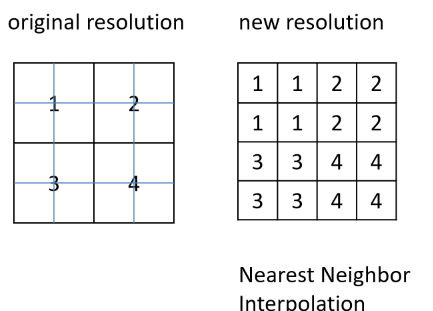
\includegraphics[width=0.4\columnwidth]{Images/nni}
\end{center}

\subsubsection{Bilinear Interpolation}
Bei vier gegeben Nachbarpunkten $Q_{11}(x_1, y_1)$, $Q_{12}(x_1, y_2)$, $Q_{21}(x_2, y_1)$ und $Q_{22}(x_2, y_2)$ können zwei Lineare Interpolationen (Nicht-Linear!) zu Endpunkt $P(x, y)$ führen.

\begin{align*}
	f(R_1=x,y_1) &\approx \frac{x_2-x}{x_2-x_1}f(Q_{11}) + \frac{x-x_1}{x_2-x_2}f(Q_{21}) \\
	f(R_2=x,y_2) &\approx \frac{x_2-x}{x_2-x_1}f(Q_{12}) + \frac{x-x_1}{x_2-x_2}f(Q_{22}) \\
	f(P) &\approx \frac{y_2-y}{y_2-y_1}f(R_1) + \frac{y-y_1}{y_2-y_1}f(R_2)
\end{align*}

\begin{center}
	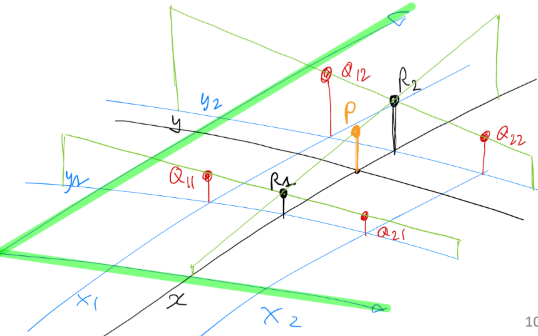
\includegraphics[width=0.7\columnwidth]{Images/bi}
\end{center}

\[
v(x, y) = ax + by + cxy + d
\]

\subsubsection{Bicubic Interpolation}
\textbf{Hinweis:} Wenn die Summe von $0$ bis $1$ geht, wird das Problem zur Bilinear Interpolation.

\[
v(x, y) = \sum_{i=0}^{3}\sum_{j=0}^{3}a_{ij}x^iy^i
\]

\subsection{Beziehung zwischen Pixeln}
Der Pixel $P$ an der Position $x,y$ hat vier Horizontal und Vertikale Nachbarn, welche als $N_4(p)$ bezeichnet sind.
\[
(x+1, y), (x-1, y), (x, y+1), (x,y-1)
\]
Die Vier Digonalen Pixeln sind als $N_D(p)$ bezeichnet.
\[
(x+1, y+1), (x-1, y-1), (x-1, y+1), (x+1,y-1)
\]
Die Komination ist $N_8(p)$ und beinhaltet alle Pixel um den Punkt $P$.

\subsection{Adjacency}
\begin{enumerate}
	\item 4-Adjazenz: Zwei Pixel $p$ und $q$ mit Werten aus $V$ sind 4-adjazent, wenn $q$ in der Menge $N_4(p)$ enthalten ist.  (Nur Gerade Verbindungen)
	\item 8-Adjazenz: Zwei Pixel $p$ und $q$ mit Werten aus $V$ sind 8-adjacent, wenn $q$ in der Menge $N_8(p)$ enthalten ist. (Alles Möglich, auch Diagonal)
	\item m-Adjazenz (gemischte Adjazenz): Zwei Pixel $p$ und $q$ mit Werten aus $V$ sind m-benachbart, wenn (Nur Ecke, wenn es nicht anders geht):
	\begin{enumerate}
		\item  $q$ ist in $N_4(p)$, oder
		\item  $q$ ist in $N_D(p)$ und die Menge $N_4(p) \cap N_4(q)$ hat keine Pixel, deren Werte aus V sind.
	\end{enumerate}
\end{enumerate}

\textbf{Beispiel:} Links ein 8-Adjazenz und rechts ein m-Adjazenz
\begin{center}
	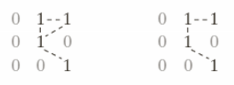
\includegraphics[width=0.4\columnwidth]{Images/adjacency}
\end{center}

\subsection{Distanzen}
Pixel $p$ und $q$ mit Koordinaten $(x, y)$ und $(s,t)$~\\


\textbf{Euclidean}
\[
D_e(p, q) = \sqrt{(x-s)^2 + (y-t)^2}
\]

\textbf{City-Block}
\[
D_4(p,q) = \left|x-s\right| + \left|y-t\right|
\]

\textbf{Chessboard}
\[
D_8(p,q) = \max\left(\left|x-s\right|, \left|y-t\right|\right)
\]

\subsection{Logical Operations}
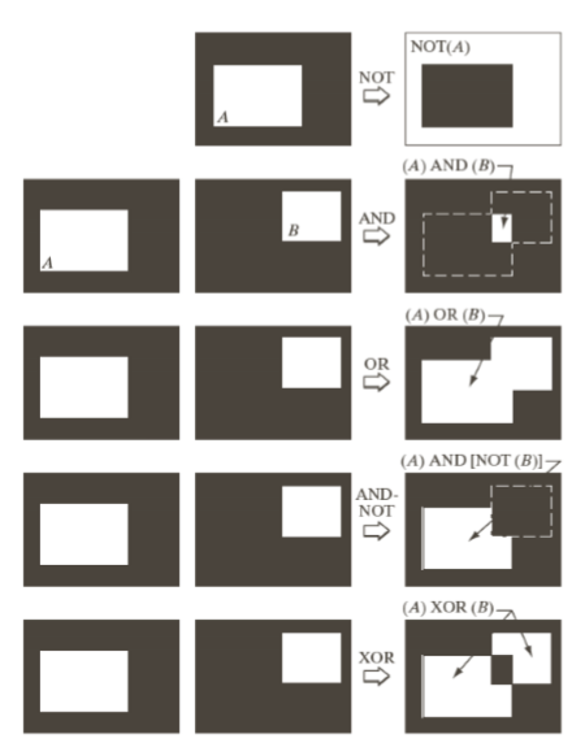
\includegraphics[width=\columnwidth]{Images/logical}

\subsection{Rauschen}
Wenn Rauschen $\mu$ im Schnitt $0$ ist und unkorreliert, dann kann dies durch Mitteln im Bild $g$ entfernt werden $\overline{g}$:
\begin{align*}
	\overline{g} &= \frac{1}{K}\sum_{i=1}^{K}g_i \\
	E\{\overline{g}\} &= g + \frac{1}{K}\sum\underbrace{ E\{\mu\}}_{=0} = g \\
	\var\{\overline{g}\} = \sigma^2_{\overline{g}} &= \frac{1}{K^2}\sum_{i=1}^{K}\underbrace{\var{\mu_i}}_{\sigma^2_n} = \frac{1}{K}\sigma^2_\mu \\
\end{align*}

\subsection{Spatial Transofmration}
\[
\begin{pmatrix}
	x^\prime \\ y^\prime \\ 1
\end{pmatrix} = \mathbf{A} \begin{pmatrix}
x \\ y \\ 1
\end{pmatrix} = \begin{pmatrix}
a_{11}  & a_{12} & a_{13}\\ a_{21}  & a_{22} & a_{23} \\ 0 & 0 & 1
\end{pmatrix} \begin{pmatrix}
x \\ y \\ 1
\end{pmatrix}
\]
Dabei ist $\mathbf{A}$ einer der folgenden Matrizen:
\begin{center}
	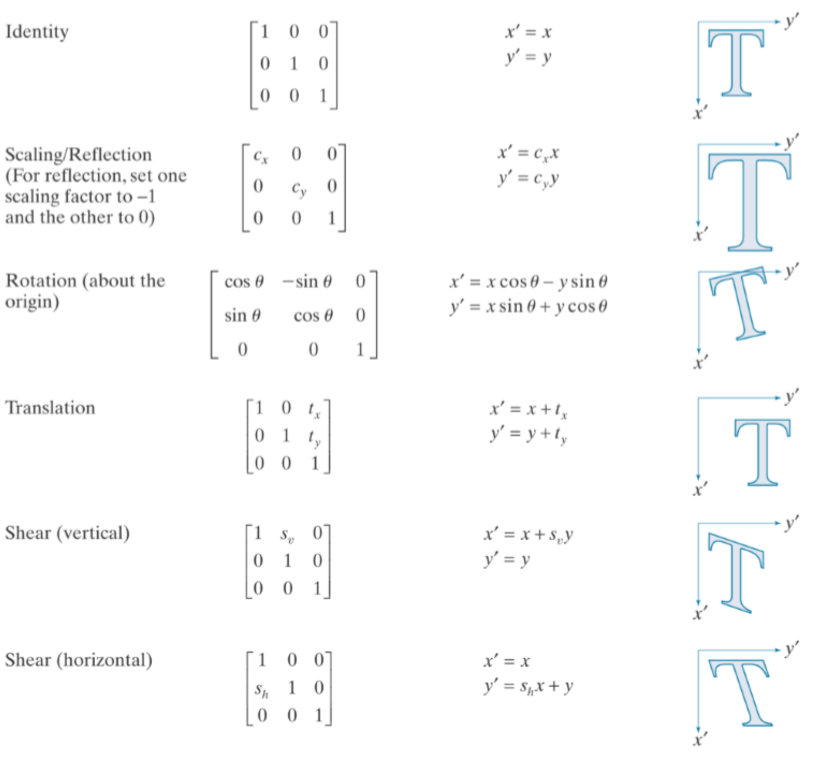
\includegraphics[width=\columnwidth]{Images/affine}
\end{center}
